% Rules for the HuroCup Basketball Competition
% Jacky Baltes <jacky@cs.umanitoba.ca> 

\documentclass[12pt]{hurocup}

\begin{document}

\title{\HuroCup: Basketball\\
  Laws of the Game 2008}


\author{Jacky Baltes\\
Autonomous Agents Laboratory\\
University of Manitoba\\
Winnipeg, Manitoba\\
Canada, R3T 2N2\\
Email: jacky@cs.umanitoba.ca\\
WWW: http://www.cs.umanitoba.ca/\~{ }jacky
}

\maketitle

\begin{center}
  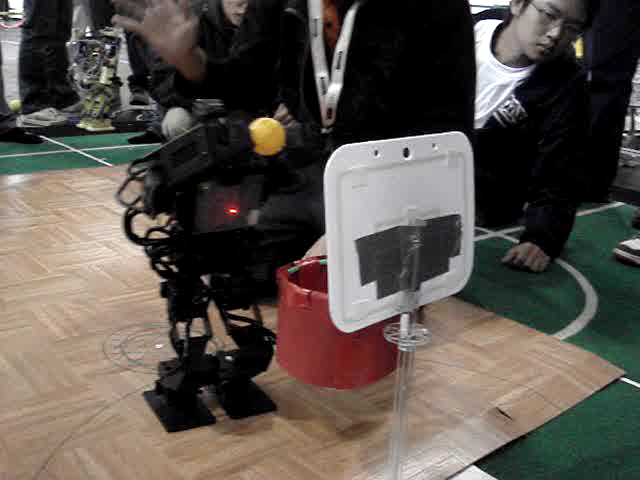
\includegraphics[width=0.7\textwidth]{Figures/basketball-life}
\end{center}

\begin{abstract}
The following rules and regulations govern the Basketball event in
\HuroCup, a robotic game and robotics benchmark problem for humanoid
robots.
%
\end{abstract}

\section*{Latest Version of the Rules for \HuroCup}
\label{sec:updates}

The latest official version of the rules of the game for \HuroCup\ is
always available from the FIRA \HuroCup\ website (http://www.fira.net).

\newpage

\section{Basketball}
\label{sec:basketball} 

The goal of the basketball competition is to encourage research into
humanoid robots that are able to dexteroursly manipulate small
objects.

\section{Changes in the Laws of \HuroCup\ for 2008}

Based on experience from the 2007 \HuroCup\ Basketball competition,
the competition was made more difficult by requiring the robot to pick
up the ball from a random position.

\section{Laws of the Game: Basketball}
\label{sec:basketball-laws}

The following laws describe the specifics of the basketball
event. For general specifications relevant to all \HuroCup\ events
(e.g., robot dimensions, playing field and lighting, responsibility of
the referees) please refer to the general \HuroCup\ laws.

\law[BB]{The Field of Play}
\label{bb-field}

\begin{lawlist}[BB]

\item The dimensions of the playing field are at least 180cm by
  180 cm (see Figure~\ref{fig:field-basketball}).

\item One side of the playing field contains a basket. This side of the
  playing field shall be called the basket side. The opposite side of
  the playing field is called the empty side. The two other sides are
  called side lines.

  \begin{figure}
    \begin{center}
      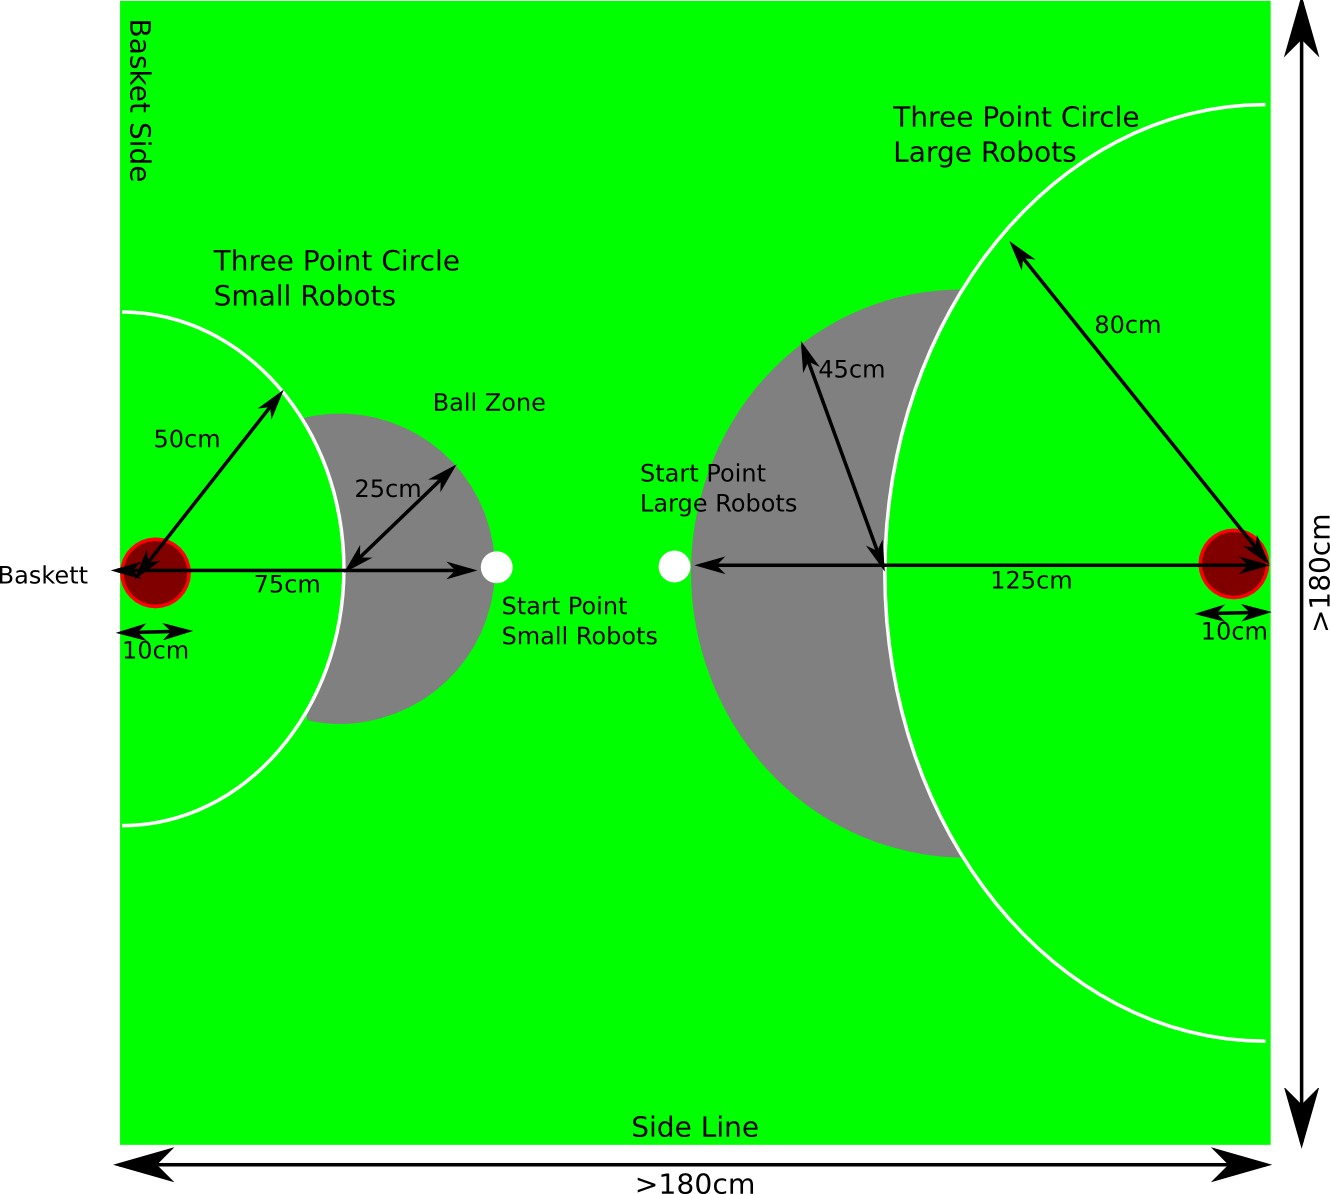
\includegraphics[width=0.7\textwidth]{Figures/basketball-field}
    \end{center}
    \caption{The field of play for basketball}
    \label{fig:field-basketball}
  \end{figure}

\item The basket is placed in the centre of the basket side.

\item A three point circle is drawn 
  \begin{itemize}
    \item 50cm away from the basket for small robots,
    \item 80cm away from the basket for large robots.
  \end{itemize}

\item The start point for
  \begin{itemize}
   \item small robots is 75cm in front of the basket in the center of
    the playing field. 
   \item large robots is 75cm in front of the basket in the center of
    the playing field.
  \end{itemize}

\item The ballzone is constructed by drawing a circle centered on the
  three point line exactly in front of the basket. The radius of the
  ballzone circle is the distance between the three point line and the
  start point for the robot. The area of this circle that is outside
  of the three point line is called the ball
  zone. Figure~\ref{fig:field-basketball} shows the ball zones for
  small and medium robots.

\end{lawlist}

\law[BB]{The Ball, Basket, and Holder}

\begin{lawlist}[BB]

  \item The ball as shown in Fig.~\ref{fig:basketball-basket} is a
  standard table tennis ball. The colour of the table tennis ball is
  either white or orange.

  \item The basket is a red coloured cup with a diameter of
  approximately 10cm and an approximate height of 10cm. The diameter
  of the bottom circle is approximately 8cm. See
  Figure~\ref{fig:basketball-basket} for an example.

  \item The top rim of the basket is mounted at a height of 25cm.

  \item The basket contains a white backboard. The backboard is 20cm
  to 25cm wide and 10cm to 15cm tall.

 \begin{figure}
    \begin{center}
      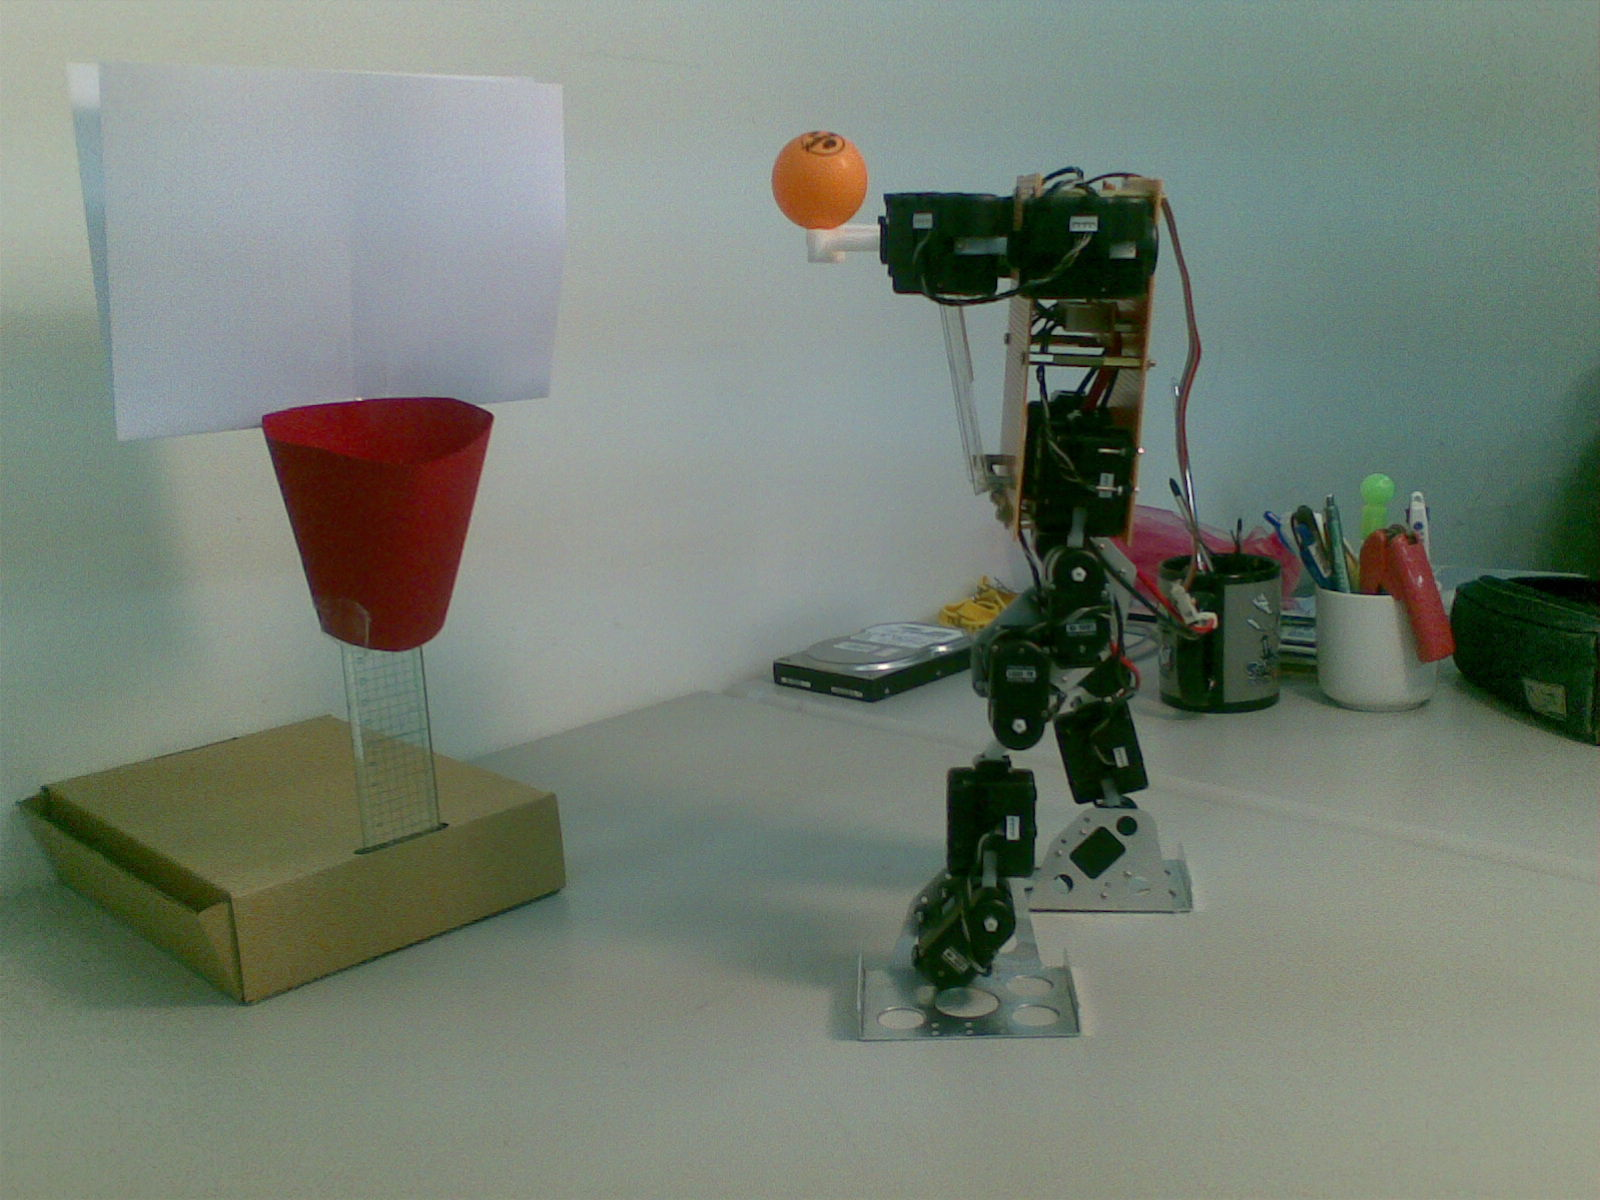
\includegraphics[width=0.7\textwidth]{Figures/basketball-basket}
    \end{center}
    \caption{A picture showing the basket ball setup. The robot is
             holding a yellow table tennis ball.}
    \label{fig:basketball-basket}
  \end{figure}

 \item A team may use a ball holder as shown in
   Fig.~\ref{fig:basketball-holder} to lift the ball off the
   ground. The diameter of the ball holder must be less than 2cm. The
   ball holder may only be used to lift the ball off the ground by a
   maximum of 20cm and the mechanics of the ball holder must not help
   the robot in any way in localizing itself or the ball. For example,
   it is forbidden to use the ball holder as a guide rail to align the
   robot with the basket.
  
 \begin{figure}
    \begin{center}
      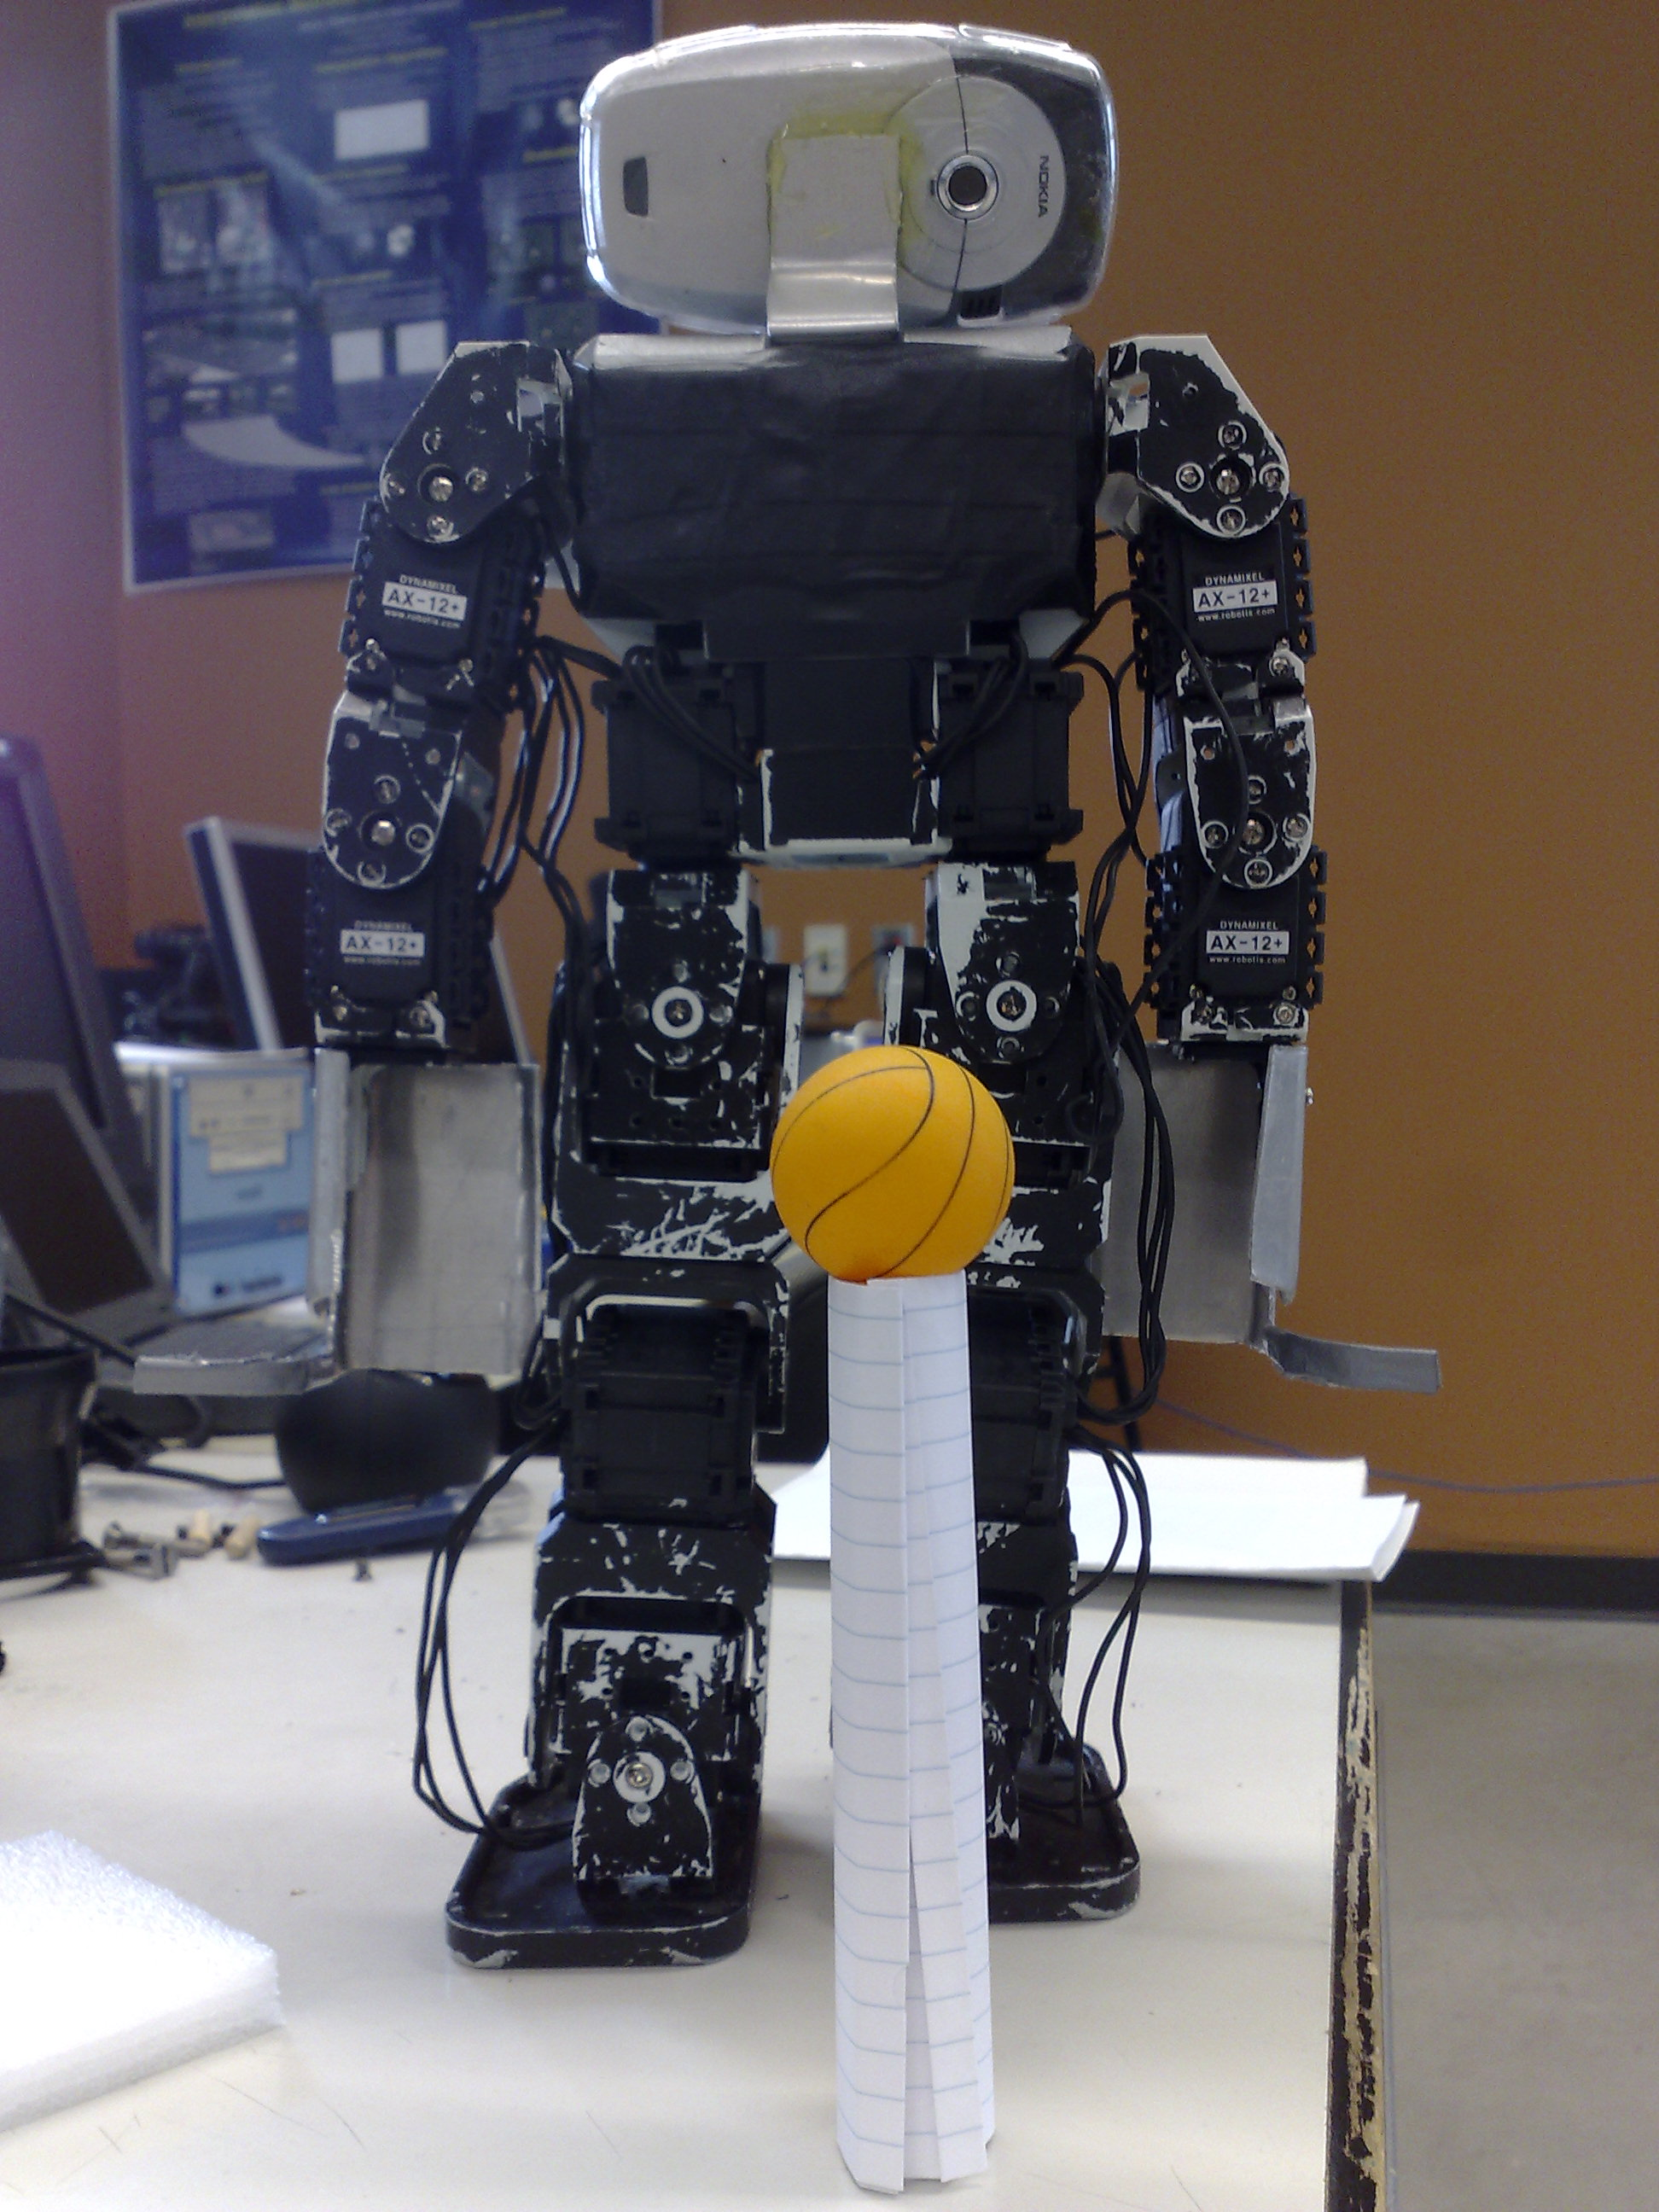
\includegraphics[width=0.7\textwidth]{Figures/basketball-holder}
    \end{center}
    \caption{A robot with a basketball holder.}
    \label{fig:basketball-holder}
  \end{figure}

 \end{lawlist}

\law[BB]{Number of Robots}

\begin{lawlist}[BB]
 \item A single robot competes in a match.
\end{lawlist}

\law[BB]{The Players}

Please refer to the general \HuroCup\ laws for a description of
the players.

\law[BB]{The Referee}

Please refer to the general \HuroCup\ laws for a description of
the referee.

\law[BB]{The Assistant Referee}

Please refer to the general \HuroCup\ laws for a description of
the assitant referee.

\law[BB]{Game Play}

\begin{lawlist}[BB]

 \item One robot is designated the thrower. All other robots must be
 positioned behind the centre line and must not interefere with the
 thrower in any way.

 \item Except the thrower, all other robots are not allowed to move
 during the throw.

 \item Each robot may have at most one human handler associated with
 it.

 \item \label{bb-handler1} The human handlers must not interfere in
 any way with other robots, the referee, or other human handlers.

 \item \label{bb-handler2} A human handler may only enter the playing
 field or touch his/her robot with the permission of the referee. The
 throw will be declared invalid if the handler touches the robot.

 \item The thrower must be at the start point at the beginning of the
 throw. 

 \item After the thrower has been placed, the referee will select a
   random position inside of the ball zone. If a team wishes to use an
   approved ball holder, the ball will be placed on the holder,
   otherwise the ball will be placed on the ground at the selected
   location.

 \item The throw begins by the referee blowing a whistle.

\item The end of the throw is signaled by the referee by
  blowing the whistle a second time.
  The referee terminates the throw if
  \begin{itemize}
  \item the ball entered the basket after being thrown by the thrower,
  \item the robot damages or moves the basket, holder, or playing
    field in any way,
  \item the ball moved outside of the playing field,
  \item a robot leaves the playing field,
  \item the maximum duration of the competition (2 minutes) has elapsed,
  \item at least 1 minute has elapsed since the start of the
    competition and it is unlikely in the opinion of the referee that
    the thrower will score in the next minute,
  \item a robot is immobilized by a technical defect.
  \end{itemize}

\item After the end of the throw, another robot is designated the
 thrower. 

\end{lawlist}

\law[BB]{Method of Scoring}
\label{basketball-scoring}

\begin{lawlist}[BB]

\item There are five rounds in the competition.

\item The three point cylinder is the volume of space described by the
 playing field as the base and extruding the three point circle
 as sides. 

\item A robot scores if the ball enters the basket, Each robot
 receives two points when any part of the robot was inside or touching
 the space of the three point cylinder when the ball was thrown. The
 robot receives three points if the robot was completely outside of
 the three point cylinder when the ball was thrown.

\item Any robot that has not scored a single point is automatically
  awarded 0 rank.

\item Among the robots that have scored at least one point, the robots
  are ranked (i.e., 1st place, 2nd place) based on the greater number
  of points that the robot scored.

\item The point allocation for robots is as follows:
  \begin{itemize}
  \item The first ranked robot is awarded $10$ points.
  \item The second ranked robot is awarded $8$ points.
  \item The third ranked robot is awarded $6$ points.
  \item The fourth, fifth, sixth, and seventh place robots are awarded
    $4$,$3$,$2$, and $1$ point respectively.  A summary of the point
    allocation for placings is shown in table~\ref{point-allocation}.

    \begin{table}
      \begin{center}
        \begin{tabular}{l|l}
          \hline
          Place & Points scored \\
          \hline
          1 (Winner) & 10 \\
          2          & 8 \\
          3          & 6 \\
          4          & 4 \\
          5          & 3 \\
          6          & 2 \\
          7          & 1 \\
          8, 9, ...  & 0 \\
          \hline
        \end{tabular}
      \end{center}
      \caption{Point allocation for placings in the \HuroCup\ events.}
      \label{point-allocation}
    \end{table}
 \end{itemize}

\item In case of a tie between $n$ robots with rank $k$, all robots
 will be awarded rank $k$ and receive the average of the scores for
 ranks $k$ to $k+n$.  For example, if the robots $A,B,C,D$ scored $10,
 8, 8, 4$ goals respectively, then robot $A$ will be declared the
 winner (1st place) and receive 10 points, both robots $B$ and $C$
 will be declared 2nd place finishers and receive $(8+6)/2=7$, and
 robot $D$ will be declared the fourth place finisher and receive $4$
 points.

\end{lawlist}

\end{document}


% *** Local Variables: ***
% *** mode: LaTeX ***
% *** mode: outline-minor ***
% *** mode: auto-fill ***
% *** mode: font-lock ***
% *** outline-regexp: "% !\\|\\\\\\(sub\\)*section" ***
% *** TeX-command-default: "LaTeX PDF" ***
% *** End: ***
